\documentclass[11pt]{article}
\usepackage[sc]{mathpazo}
\usepackage{amsmath,pifont}
\usepackage{fullpage}
\usepackage[authoryear,sectionbib,sort]{natbib}
\linespread{1.7}
\usepackage[utf8]{inputenc}
\usepackage{lineno}

\usepackage{graphicx} 
\usepackage{tabularx,setspace}

\title{Density-dependent selection and the population ecology of relative fitness}
%\author{Jason Bertram $^{1,\ast}$ \\ 
%Joanna Masel $^{1}$}

\date{}

\begin{document}

\maketitle

%\noindent{}1. Department of Ecology and Evolutionary Biology, University of Arizona, Tucson, AZ 85721.

%\noindent{}$\ast$ Corresponding author; e-mail: jbertram@email.arizona.edu.


\bigskip

%\textit{Manuscript elements}: 

\bigskip

\textit{Keywords}: $r$/$K$ selection, absolute fitness, eco-evo, competition-colonization trade-off, fluctuating selection, storage effect.

\bigskip


\linenumbers{}
\modulolinenumbers[1]

\newpage{}

\section*{Abstract}


new model of density-dependent selection by generalizing the fixed-density classic lottery model of territorial acquisition to accommodate arbitrary population densities. 

We show that, with density dependence, co-existence is possible in the lottery model in a stable environment. 

Inspired by natural \textit{Drosophila} populations, we consider co-existence under strong, seasonally-fluctuating selection coupled to large cycles in population density, and show that co-existence (stable polymorphism) is promoted via a combination of the classic storage effect and density-regulated population growth. 

\newpage{}


\section*{Introduction}

There are a variety of different measures of fitness. Some widely used examples in evolutionary ecology are expected lifetime reproductive ratio $R_0$, intrinsic growth rate $r$, saturation population density (often labeled ``$K$'') \citep{benton_2000}, and invasion fitness \citep{metz_1992}. In addition, ``relative fitness'' is the standard in much of evolutionary biology, particularly evolutionary genetics, where attention is generally restricted to relative genotypic proportions \cite[pp. 468]{barton_2007}. This variety is not necessarily problematic in itself, because different measures of fitness may be more useful in different circumstances. But any measure of fitness should ultimately be grounded in the processes of birth and death which govern population biology \citep{metcalf_2007,doebeli_2017}. While this grounding is clear for absolute fitness measures like $r$ and $K$, relative fitness seems largely divorced from population ecology.

In uncrowded populations, relative fitness simply represents differences in the intrinsic exponential growth rate $r$ \citep[pp. 26]{crow_1970}, with selection favoring greater $r$ ($r$-selection). In crowded populations, relative fitness models almost universally assume that total population size $N$ is fixed, or has some externally imposed time course. This is exemplified by the Wright-Fisher model, in which time advances in discrete non-overlapping generations, and fitness can be interpreted as a product of fertility and juvenile viability \citep[pp. 185]{crow_1970}. The limitations of these relative fitness models are openly acknowledged, usually with an emphasis on the difficulty of incorporating more of the life cycle ``components'' of fitness (e.g. \cite[pp. 276]{ewens_2004}). But more fundamentally, the constant-$N$, relative fitness description uncouples selection and demography, at odds with the fact that the same birth/death events drive both. 

The issue can be expressed more formally by revisiting MacArthur's analysis of selection in crowded populations \citep{macarthur_1967}. MacArthur considers a population consisting of two types with densities $n_1$ and $n_2$ subject to density-dependent population growth described by
\begin{equation}
\frac{d n_1}{d t}=f_1(n_1,n_2)\qquad\frac{d n_2}{d t}=f_2(n_1,n_2). \label{eq:macgeneral}
\end{equation}
Other than densities, the environment is assumed to remain constant. The functions $f_1$ and $f_2$ must decline to zero if $n_1$ or $n_2$ are sufficiently large, because no population has unlimited resources. This defines the nullclines $f_1(n_1,n_2)=0$ and $f_2(n_1,n_2)=0$ in $(n_1,n_2)$ space. The outcome of selection is then determined by the relationship between these nullclines. Specifically, a type will be excluded if its nullcline is completely contained in the region bounded by the other type's nullcline. In other words, for a type to have the possibility of persisting, it must be able to keep growing to higher densities than the other type can tolerate in some region of $(n_1,n_2)$ space (Fig.~\ref{fig:Ksel}a). 

This conclusion about selection in crowded populations does not seem compatible with the constant-$N$ assumption of relative fitness models. The incompatibility is particularly apparent in some of the most widely-used models of density-regulated population growth (to illustrate our point we stick to the simple haploid case): 1) The logistic model: the type with the greatest saturation population density excludes the others. 2) The ``$R^*$ rule'', a central tenet of resource competition theory, states that when multiple types are exploiting a homogeneous consumable resource that limits their growth, the type able to deplete the resource to the lowest equilibrium density $R^*$ excludes the others \citep{grover_1997}. Except in special cases, differences in $R^*$ entails differences in saturation population density. 3) The Lotka-Volterra competition model also couples selection in crowded populations to changes in total density $N$ (we return to this in BLAH). Thus, it would seem that the ubiquitous constant-$N$, relative fitness description of selection is incompatible with a huge class of population ecological processes occurring in nature and experiments. 

It is not even clear how to connect relative fitness models to density-regulated growth, since they only describe selection along lines defined by $n_1+n_2=N$ for each $N$ (Fig.~\ref{fig:Ksel}b); the $f_1$ and $f_2$ nullclines are thus not defined.

\begin{figure}
\centering
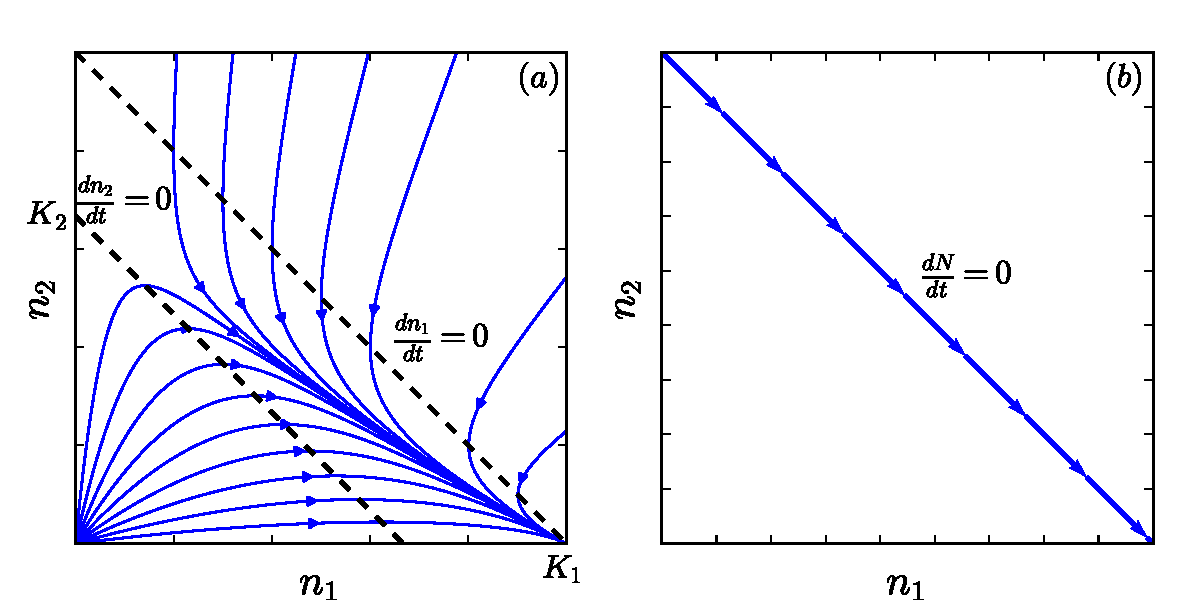
\includegraphics[scale=0.8]{Kplot.pdf}
\caption{\label{fig:Ksel} (a) MacArthur's dynamical argument for how selection operates in crowded environments, illustrated using the logistic model $f_1=r_1(1-\frac{n_1+n_2}{K_1})n_1$ and $f_2=r_2(1-\frac{n_1+n_2}{K_2})n_1$ in Eq. \eqref{eq:macgeneral}. Here $r_1=r_2$ and $K_1>K_2$. (b) The constant-$N$, relative fitness description of selection.}
\end{figure}

The constant-$N$, relative fitness description has historically been justified as a short-term linear approximation of a more complicated long-term eco-evolutionary process \cite[pp. 277]{ewens_2004}. That is, within a sufficiently short time frame, population size can be treated as constant and selection quantified in terms of constant selection coefficients expressing relative fitness differences. Provided that selection is sufficiently weak and stable over time, this ``short-term''  assumption is not a major restriction. Yet it is increasingly recognized that selection is not always weak, that it can fluctuate dramatically over time, and coupled to this, that a population's density can vary by orders of magnitude over a few generations as a routine feature of its ecology. These are not rare exceptions, but occur widely in nature and the lab, including in wild \textit{Drosophila} \citep{messer_2016}. Moreover, the short-term approximation automatically precludes consideration of inherently long-term evolutionary processes like the management of genetic load and population extinction \citep{bertram_2017}. Nevertheless, relative fitness models like Wright-Fisher are the foundation for much of the population genetic literature, and are still widely used without considering the ``short-term'' restriction. Thus, to summarize, there are important theoretical and practical reasons to deepen our understanding of the population-ecological foundations of relative fitness models.

Here we introduce a novel model of density-dependent population growth based on territorial contests, and show that when this model reaches a demographic steady-state, the constant-$N$, relative fitness picture emerges. Our model is firmly grounded in population ecology, with fundamental parameters given by birth and death rates, and competitive ability. We show that this model can also be interpreted as a density-dependent generalization of the Wright-Fisher model with overlapping generations. 

Futhermore, we show that our model is entirely consistent with MacArthur's analysis of selection in crowded populations. In particular, we emphasize that MacArthur's argument does not justify the widespread intuition that selection in crowded environments is necessarily connected to achieving greater densities \citep{anderson_1971}. This is largely an artifact of the models historically used in the density-dependent selection literature, which ignore relative contests. 

%This  also seems to be why the density-dependent selection literature expended such considerable effort to showing that evolution under density-dependent selection optimizes population size in some sense \citep{roughgarden_1979} --- a meaningless

Our model is essentially a density-dependent generalization of the classic ecological lottery model \cite{chesson_1981}. In the lottery model, mature individuals (``adults'') each require their own territory, whereas newborn individuals (``propagules'') disperse to, and subsequently compete for, territories made available by the death of adults. Territorial contest among propagules leaves a single victorious adult per territory, the victor chosen at random from the propagules present, with probabilities weighted by a coefficient for each type representing competitive ability, akin to a weighted lottery \citep{sale_77}.  

The classic lottery model assumes a saturated population with constant $N$, and a large number of propagules dispersing to each territory (the Wright-Fisher model makes a similar ``infinite propagule'' assumption to justify sampling with replacement). As such, the lottery model breaks down at low densities (few propagules dispersing to each territory). Our first task is to analytically extend the classic lottery model to correctly account for low density behavior (sections ``Model'' and ``Mean field approximation''). We then...

 
\section*{Model}\label{sec:model}

\subsection*{Basic assumptions}

We assume that reproductively mature individuals (``adults'') each require their own territory to survive and reproduce (Fig.~\ref{fig:lottery}). All territories are identical, and the total number of territories is $T$. Time $t$ advances in discrete iterations, each representing the time from birth to reproductive maturity. In iteration $t$, the number of adults of the $i$'th type is $n_i(t)$, the total number of adults is $N(t)=\sum_i n_i(t)$, and the number of unoccupied territories is $U(t)=T-N(t)$. 

We assume that the $n_i$ are large enough that stochastic fluctuations in the $n_i$ (``drift'') can be ignored. In particular, we do not evaluate the initial stochastic behaviour of mutant lineages while they are at low abundance. We derive deterministic equations for the expected change in the $n_i$ over time, leaving the evaluation of drift for future work.  

%When considering new mutations, we therefore restrict our attention to the earliest (lowest $n_i$) deterministic behavior of mutant lineages (the transition to deterministic growth occurs at an abundance $n_i$ of order equal to their inverse expected absolute growth rate; \citealt{uecker_2011}).

\begin{figure}
\centering
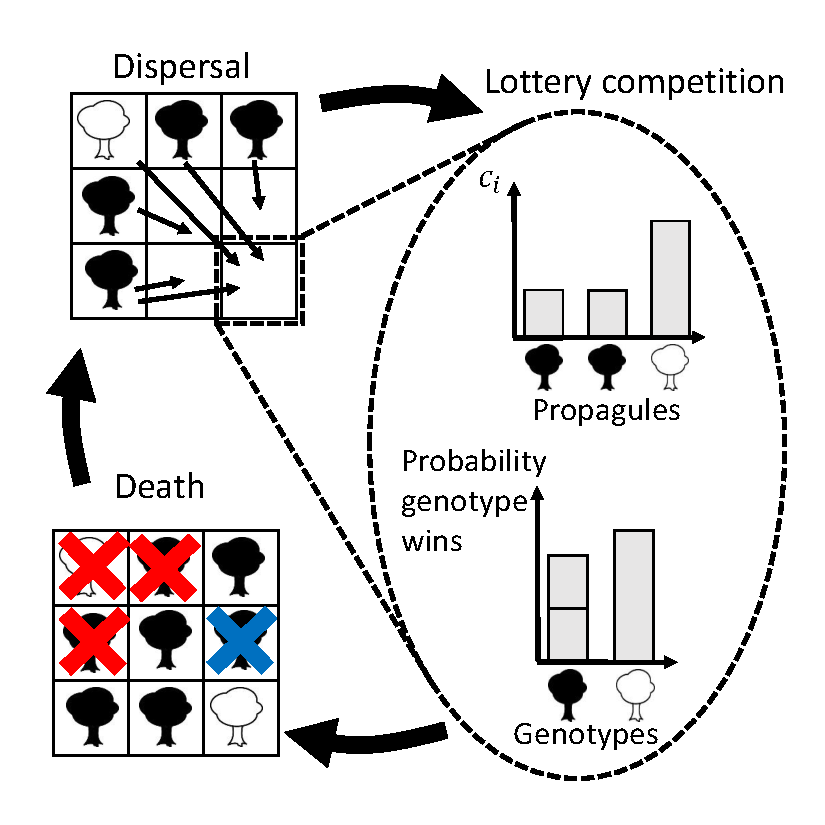
\includegraphics[scale=0.8]{lottery.pdf}
\caption{\label{fig:lottery} Each iteration of our model has three elements. First, propagules are produced by adults and dispersed at random (only propagules landing on unoccupied territories are shown). Some territories may receive zero propagules. Lottery competition then occurs in each unoccupied territory that receives a propagule (only illustrated in one territory). Each type has a probability proportional to $c_i x_i$ of securing a given territory, where $c_i$ measures competitive ability and $x_i$ is the number of propagules that disperse there. In the illustrated territory, the black type disperses more propagules but is a poorer competitor. Territories are then made available by deaths among those adults present at the start of the iteration (red crosses).}
\end{figure}

Each iteration, adults produce new offspring (``propagules''), $m_i$ of which disperse to unoccupied territories. We assume that adults cannot be ousted from their territories, so that $m_i$ only includes propagules landing on unoccupied territories. Propagules disperse at random over the unoccupied territories, regardless of distance from their parents, and independently of each other. There is no interaction between propagules (e.g. avoidance of territories crowded with propagules). Loss of propagules during dispersal is subsumed into $m_i$. We assume that each adult produces a constant number $b_i$ of successfully dispersing propagules; the loss of propagules due to dispersal to occupied territories then implies $m_i=b_i(1-N/T)n_i$. Note that due to our assumption of uniform dispersal, the parameter $b_i$ can be thought of as a measure of ``colonization ability'', which combines fecundity and dispersal ability \citep{levins_71,tilman_94,bolker_99}. In addition to random dispersal, we will compare our model to perfect directed dispersal, in which each propagule finds an unoccupied territory if one is available ($m_i=b_i$) \citep{chesson_1983}. 

The number of individuals of the $i$'th type landing in any particular territory is denoted $x_i$. We assume that $x_i$ follows a Poisson distribution $p_i(x_i)=l_i^{x_i} e^{-l_i}/x_i!$, where $l_i=m_i/U$ is the mean territorial propagule density. This is approximation becomes exact when the $n_i$ are large enough that drift in $n_i$ can be ignored (Appendix A).

When multiple propagules land on the same territory, the victor is determined by lottery competition: type $i$ wins a territory with probability $c_i x_i/\sum_j c_j x_j$, where $c_i$ is a constant representing relative competitive ability (Fig. \ref{fig:lottery}). We expect that a fraction $p_1(x_1)\ldots p_G(x_G)$ of the $U$ unoccupied territories will have the propagule composition $x_1,\ldots,x_G$. type $i$ is expected to win $c_i x_i/\sum_j c_j x_j$ of these. Ignoring fluctuations about these two expectations (due to our no-drift, large $T$, large $n_i$ approximation), type $i$'s territorial acquisition is given by
\begin{equation}
\Delta_+ n_i(t)=U(t)\sum_{x_1,\ldots,x_G} \frac{c_i x_i}{\sum_j c_j x_j} p_1(x_1)\ldots p_G(x_G), \label{eq:growthsumuncoupled}
\end{equation}
in our extended lottery model, where the sum only includes territories with at least one propagule present.

Finally, we assume that mortality only occurs in adults (Fig.~\ref{fig:lottery}; setting aside the juvenile deaths implicit in territorial contest), and at a constant, type-specific per-capita rate $0\leq d_i\leq 1$, so that the overall change in type abundances is
\begin{equation}
\Delta n_i(t)=\Delta_+ n_i(t)-d_i n_i(t). \label{eq:delttot}
\end{equation}

\subsection*{Connection to the Wright-Fisher and classic lottery models}

In the classic lottery model \citep{chesson_1981}, unoccupied territories are assumed to be saturated with propagules from every type $l_i\gg 1$. From the law of large numbers, the composition of propagules in each territory will then not deviate appreciably from the mean composition $l_1,l_2,\ldots,l_G$ ($G$ is the number of types present), and so the probability that type $i$ wins any particular unoccupied territory is approximately $c_i l_i/\sum_j c_j l_j$. Then the numbers of territories won by each type $\Delta_+ n_1,\Delta_+ n_2,\ldots,\Delta_+ n_G$ follow a multinomial distribution with $U$ trials and success probabilities $\frac{c_1 l_1}{\sum_j c_j l_j},\frac{c_2 l_2}{\sum_j c_j l_j},\ldots,\frac{c_G l_G}{\sum_j c_j l_j}$, respectively. Type $i$ is expected to win $c_i l_i/\sum_j c_j l_j$ of the $U$ available territories, and deviations from this expected outcome are small (since $T$ is large by assumption), giving 
\begin{equation}
\Delta_+ n_i(t)=\frac{c_i l_i}{\sum_j c_j l_j}U(t)=\frac{c_i l_i}{\overline{c}L}U(t), \label{eq:lottery}
\end{equation}
where $\overline{c}=\sum_j c_j m_j/M$ is the mean propagule competitive ability for a randomly selected propagule, $L=M/U$ is the total propagule density and $M=\sum_j m_j$ is the total number of propagules. 

Eq. \eqref{eq:lottery} breaks down for types with low propagule density ($l_i\ll 1$) because territorial acquisition is then not correctly represented by a lottery in each territory with the mean propagule density. Instead, a rare type's propagules only make it to a few territories where at least one of its propagule present. In our extension of the classic lottery model, we correct (Eq.~\ref{eq:delttot}) to account for this.

%type $i$ can win at most $m_i$ territories, yet Eq.~\eqref{eq:lottery} demands $c_i l_i/\sum_j c_j l_j$ of the $U$ unoccupied territories, for any value of $U$.
 
There is a close connection between the classic lottery model and the Wright-Fisher model of genetic drift \citep{svardal_2015}. In the Wright-Fisher model, type abundances are sampled each generation from a multinomial distribution with success probabilities $w_i n_i/\sum_j w_j n_j$, where $w$ is relative fitness and the $n_i$ are  type abundances in the preceding generation. Population size $N$ remains constant. This is equivalent to the classic lottery model with non-overlapping generations ($d_i=1$ for all $i$) and relative fitness given by $w_i=b_i c_i$ i.e. a product of fecundity and viability \citep[pp. 185]{crow_1970}. Thus, the classic lottery model is essentially the Wright-Fisher model extended to allow overlapping generations, but ignoring drift. This means that our extension of the classic lottery model to arbitrary densities represents a density-dependent generalization of the Wright-Fisher model.

\section*{Results}

\subsection*{Mean Field Approximation}

Eq. \eqref{eq:growthsumuncoupled} involves an expectation over the time-dependent dispersal distributions $p_i$, and is thus too complicated to give intuition about the dynamics of density-dependent lottery competition. We now evaluate this expectation using a ``mean field'' approximation. 

Similarly to the high-$l_i$ approximation of classic lottery model, we replace the $x_i$ with appropriate mean values, although we cannot simply replace $x_i$ with $l_i$. For a type with low propagule density $l_i\ll 1$, we have $x_i=1$ in the territories where its propagules land, and so its growth comes entirely from territories which deviate appreciably from $l_i$. To account for this, we separate Eq. \eqref{eq:growthsumuncoupled} into $x_i=1$ and $x_i>1$ parts. Our more general mean field approximation only requires that there are no large discrepancies in competitive ability (i.e. we do not have $c_i/c_j\gg 1$ for any two types). We obtain (details in Appendix B)
\begin{equation}
\Delta_+ n_i(t)\approx \left[e^{-L}+(R_i+A_i)\frac{c_i}{\overline{c}}\right]l_i U(t), \label{eq:master}
\end{equation}
where
\begin{equation}
R_i=\frac{\overline{c}e^{-l_i}(1-e^{-(L-l_i)})}{c_i +\frac{\overline{c}L- c_il_i}{L-l_i}\frac{L-1+e^{-L}}{1-(1+L)e^{-L}}},\label{eq:Dr}
\end{equation}
and
\begin{equation}
A_i=\frac{\overline{c}(1-e^{-l_i})}{\frac{1-e^{-l_i}}{1-(1+l_i)e^{-l_i}}c_il_i+\frac{\overline{c}L- c_il_i}{L-l_i}\left(L\frac{1-e^{-L}}{1-(1+L)e^{-L}}-l_i\frac{1-e^{-l_i}}{1-(1+l_i)e^{-l_i}}\right)}.\label{eq:Da}
\end{equation}

Comparing Eq. \eqref{eq:master} to Eq. \eqref{eq:lottery}, the classic lottery per-propagule success rate $c_i/\overline{c}L$ has been replaced by three separate terms. The first, $e^{-L}$, accounts for propagules which land alone on unoccupied territories; these territories are won without contest. The second, $R_i c_i/\overline{c}$ represents competitive victories when the $i$ type is a rare invader in a high density population, determining its invasion fitness \citep{metz_1992}. The third term, $A_i c_i/\overline{c}$, represents competitive victories when the $i$ type is abundant. The relative importance of these three terms varies with both the overall propagule density $L$ and the relative propagule frequencies $m_i/M$. If $l_i\gg 1$ for all types, we recover the classic lottery model (only the $A_ic_i/\overline{c}$ term remains, and $A_i\rightarrow 1/L$). Note that not all unoccupied territories are claimed each iteration, since under Poisson dispersal a fraction $e^{-L}$ remain unoccupied; the total number of territories gained is thus $\Delta_+ N=U(1-e^{-L})$.

Fig.~\ref{fig:simcomp} shows that Eq. \eqref{eq:master} and its components closely approximate individual-based simulations of the density-dependent lottery model over a wide range of propagule densities $l_i$. Two types are present, one of which is at low frequency. The growth of the low-frequency type relies crucially on the low-density competition term $R_i c_i/\overline{c}$. On the other hand, $R_i c_i/\overline{c}$ is negligible for the high-frequency type, which depends instead on high density territorial victories. Fig.~\ref{fig:simcomp} also shows the breakdown of the classic lottery model at low propagule densities.

\begin{figure}
\centering
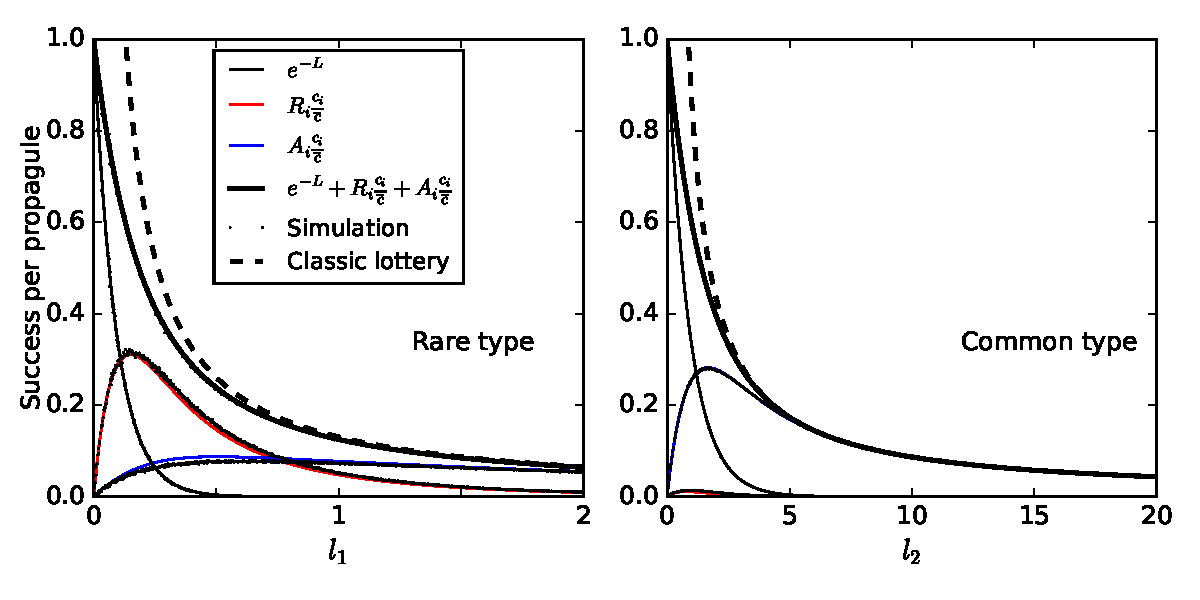
\includegraphics[scale=0.8]{simulationcomparison.pdf}
\caption{\label{fig:simcomp} Comparison of mean field approximation Eq. \eqref{eq:master} with simulations. Per-propagule success probability $\Delta_+ n_i/l_i U$ from the classic lottery model, individual-based simulations of random dispersal and lottery competition, and Eq. \eqref{eq:master} and its three components. Two types are present, a rare type with $c_1=1.5$, and a common type with $c_2=1$. Simulation points are almost invisible in for the common type due to near exact agreement with Eq. \eqref{eq:master}. Dashed lines in show the breakdown of the classic lottery model. Parameters: $m_1=10^4$ and $m_2=9\times 10^4$ and $U$ is varied between $5\times 10^3$ and $10^6$.} 
\end{figure}

\subsection*{$K$-selection, $c$-selection and relative fitness}

We now compare MacArthur's claims about selection in crowded environments with our density-dependent lottery model.

--- commonly referred to as ``$K$-selection'' (Fig.~\ref{fig:Ksel}a)


As shown in the Introduction, MacArthur's argument revolves around the behaviour of  ecological models of the general form Eq.~\ref{eq:macgeneral}, which depends on the relationship between the nullclines $f_1(n_1,n_2)=0$ and $f_2(n_1,n_2)=0$. To formalize this relationship, MacArthur used the symbol ``$K$'' to label the four intersection points of the nullclines with the $n_1$ and $n_2$ axes, specifically $f_1(K_{11},0)=0$, $f_1(0,K_{12})=0$, $f_2(0,K_{22})=0$ and $f_2(K_{21},0)=0$. These $K$ values determine whether a region of higher-density growth exists for each type, provided that the nullclines are close to being straight lines. Note that only $K_{11}$ and $K_{22}$ are saturation densities akin to the $K$ parameter in the logistic model; $K_{12}$ and $K_{21}$ are related to competition between types. For instance, in the Lotka-Volterra competition model we have $f_1(n_1,n_2)=r_1(1-\alpha_{11}n_1-\alpha_{12}n_2)n_1$ where $\alpha_{11}=1/K_{11}$ measures competitive effects within the first type, whereas $\alpha_{12}=1/K_{12}$ measures competitive effects on the first type due to the second (Fig.~\ref{fig:LVvslottery}a). Thus, when MacArthur concludes that  ``fitness is $K$'' in crowded populations \citep[pp. 149]{macarthur_1967}, the meaning is that selection either favors the ability to keep growing at ever higher densities (moving a type's own nullcline outwards), or the ability to suppress the growth of competitors at lower densities (moving the nullcline of competitors inwards). This general idea applies even if the nullclines are nonlinear to such an extent that the ``$K$'' values themselves do not give much information about the regions of high-density growth.

\begin{figure}
\centering
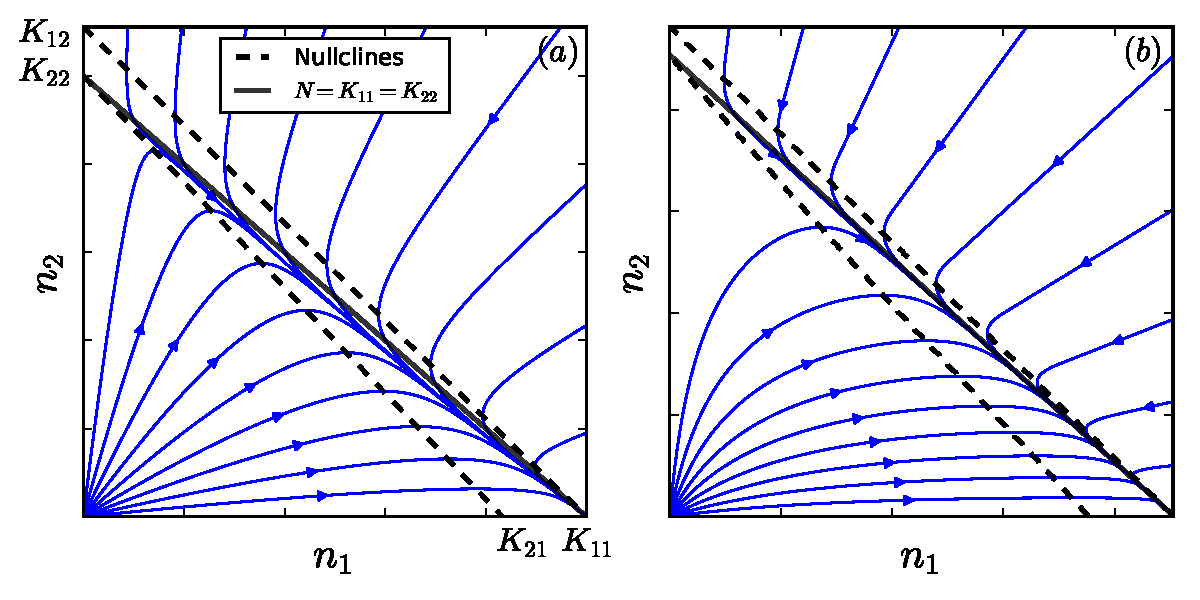
\includegraphics[scale=0.8]{LVvslottery.pdf}
\caption{\label{fig:LVvslottery} Blah}
\end{figure}

In Fig.~\ref{fig:LVvslottery} we show a phase diagram for Eq.~\eqref{eq:master} 


\subsection*{Coexistence in constant and cyclical environments}\label{sec:invas}

In the previous section we only considered how $b$, $c$ and $d$ should respond to selection in Grime's environmental extremes, based on invasion fitness. Here we further explore the low frequency behavior of Eq. \eqref{eq:master} to determine which types can coexist in a constant environment, and then consider the full time-dependent behaviour of Eq. \eqref{eq:master} in a cyclical environment. 

In a constant environment, stable coexistence is possible in our extended lottery model. A $b$-specialist $i$ and $c$-specialist $j$ ($b_i>b_j$, $c_j>c_i$) can co-exist because then propagule density $L$ is frequency-dependent, and so is the importance of competitive ability (Appendix D). This is a version of the classic competition-colonization trade-off \citep{tilman_94,levins_71}; the competitor ($c$-specialist) leaves many territories unoccupied (low $L$) due to its poor colonization ability (low $b$), which the colonizer ($b$-specialist) can then exploit. A similar situation holds for coexistence between high-$c$ and low-$d$ specialists; a ``competition-longevity'' trade-off \citep{tilman_94}. These forms of co-existence require density dependence (being mediated by $L$), and are not present in the classic lottery model. Coexistence is not possible between $b$- and $d$-specialists in a constant environment (Appendix D). 

Now suppose that birth and death rates vary periodically with amplitude sufficent to cause large changes in population density. This example is inspired by natural \textit{Drosophila} populations, which expand rapidly in the warmer months when fruit is abundant, but largely die off in the colder months. Along with this seasonal population density cycle, hundreds of polymorphisms exhibit frequency cycles that are in phase with the seasons \citep{bergland_14}. Some of these polymorphisms may be adaptive and potentially millions of years old, suggesting stable coexistence \citep{bergland_14,messer_2016}. Selection on allele frequencies thus occurs on the same time scale as population demography, a situation vastly more complicated than classical sweeps in demographically stable populations \citep{messer_2016}.

The classical population genetic treatment of fluctuating selection suggests that environmental fluctuations do not promote coexistence. Allele frequencies are successively multiplied by relative fitness values for each environmental iteration, and so two alleles favored in different environments can only stably coexist if the product of fitnesses for one type exactly equals the product for the other \citep{dempster_1955}. Thus, stable coexistence still requires frequency-dependent selection or heterozygote advantage (as is required in a constant environment). 

This classical argument overlooks two general mechanisms that promote coexistence in fluctuating environments \citep{messer_2016}. The first is the classic version of the storage effect, which occurs when part of the population is protected from selection (due to overlapping generations in the lottery model; \citealt{chesson_1981}). The second is the bounded population size effect of \cite{yi_2013}, which occurs when each environmental cycle involves growth from low to high density, with the time spent growing each cycle dependent on the fitness of the types present. 

Fig.~\ref{fig:fluctuatingselection}a-c shows the behavior of Eq. \eqref{eq:master} for an example where $b$ and $d$ cycle between zero and positive values (``summers'' with rapid growth and no mortality, and ``winters'' with mortality and no growth). Both the storage effect (adults are sheltered from selection during the summer growth phase) and the bounded density effect (expansion to high density occurs every cycle) are operating. Two types are present, a $b$-specialist, which is better at rapidly growing in the summer (higher $b$), and a $d$-specialist which is better at surviving the winter (lower $d$). Neither type has an advantage over a full environmental cycle, and they stably coexist. This is due to a combination of the storage and bounded density effects (recall that stable coexistence between $b$ and $d$ specialists was not possible in a constant environment). 

The classic lottery model (Eq. BLAH) fails to give co-existence for these parameters because expansion to carrying capacity occurs immediately at the start of the summer (Fig. \ref{fig:fluctuatingselection}d-f). As a result, coexistence requires that the winter survivor's $b$ must be about $5$ times smaller than required when we properly account for the growth in the abundance of each type using Eq. \eqref{eq:master} (keeping the other parameters the same; Fig.~\ref{fig:fluctuatingselection}g-i). Previous models of the promotion of genetic variation via the storage effect  \citep{ellner_1994} similarly assume that the total number of offspring per iteration is constant, and would produce a similar error. 

\begin{figure}
\centering
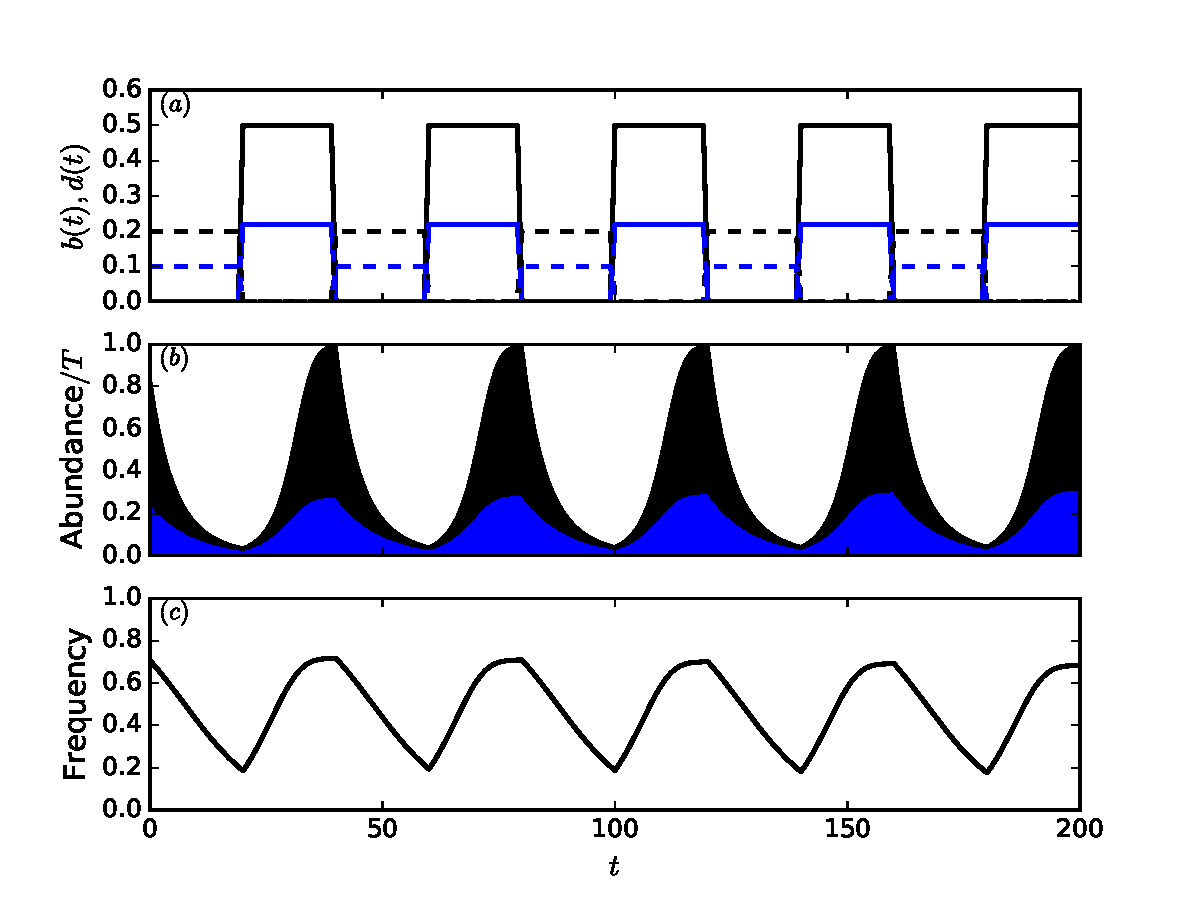
\includegraphics[scale=0.7]{fluctuatingselection.pdf}
\caption{\label{fig:fluctuatingselection} Stable coexistence between $b$ and $d$ specialists in a fluctuating environment requires a much greater $b$ advantage in the classic lottery model compared to our density-dependent extension of it when population density is seasonally cyclical. (a) Birth and death rates seasonally alternate being nonzero (white for winter, green for summer). The $b$-specialist (black) has higher $b$ and $d$ ($b=0.5$, $d=0.2$) than the $d$-specialist ($b=0.217$, $d=0.1$) (blue). (b) Both types grow during the positive $b$ phase, and decline during the positive $d$ phase, but the $d$-specialist does so at a lower rate. Total height (blue+black) is population density $N/T$. (c) Summer favors the $b$ specialist, winter the $d$-specialist, and they stably coexist. (d-f) Same as (a-c) for the classic lottery model; the types no longer coexist. (g-i) Same as (d-f) where now $b = 0.0421$ for the $d$ specialist and the types coexist. For illustration, the propagule abundances are assumed to have the form $m_i=b_i(1-N/T)n_i$, reflecting non-directed dispersal.} 
\end{figure}




\section*{Discussion}

It is interesting to compare the predictions of the extended lottery model with earlier approaches, such as the $r$/$K$ scheme, where $r=b-d$ is the maximal, low-density growth rate \citep{pianka_1972}. Confusingly, the term ``$K$-selection'' sometimes refers generally to selection at high density \citep{pianka_1972}, encompassing both selection for higher saturation density \citep{macarthur_1967} and competitive ability \citep{gill_1974}. Contrary to predictions of an $r$/$K$ trade-off, empirical studies have shown that maximal growth rate at low density and the high density at which saturation occurs (measured by abundance) are positively correlated, both between species/strains \citep{luckinbill_1979,kuno_1991,hendriks_2005,fitzsimmons_2010}, and as a result of experimental evolution \citep{luckinbill_1978,luckinbill_1979}. From the perspective of our model, this positive correlation is not surprising since the saturation density, which is determined by a balance between births and deaths, increases with $b$. 

%This prediction is also counter to the expectations of MacArthur's $r$/$K$ dichotomy \citep{macarthur_1967}, since $b$ is closely related to the maximal, low-density growth rate $r=b-d$ \citep{pianka_1972}, yet in the $r$/$K$ scheme, high density populations should be subject to $K$, not $r$, selection. Yet it is not surprising that $b$ can matter at high densities. In our model (or any lottery model of competition), $b$ matters at high densities because territorial contests among juveniles are intrinsically unpredictable. This is a realistic feature of the model. Even if one type is guaranteed to win a territory in a ``fair'' contest (e.g. it is the most efficient exploiter of a limiting consumable resource; \citealt{tilman_1982}), inferior competitors can win by chance. For example, an inferior competitor's propagules may happen to arrive first, gaining a decisive developmental advantage. First arrivals are more likely to occur for types with a fecundity and/or dispersal advantage, as represented by higher $b$ in lottery models. The analogous intuition in the Wright-Fisher model is that fecundity confers a relative fitness advantage, even though population size is not changing. The logistic model for which $r$ and $K$ are named, does not capture this intuition. 

%In fact, one step in MacArthur's argument considerably narrows its scope: assuming that the nullclines of $f_1$ and $f_2$ exist at all. The strength of this assumption is clear if we note that essence of the dichotomy underlying the $r$/$K$ scheme is between interaction-dependent selection and interaction-independent selection. That is, selective shifts in frequency are a result of differences in absolute growth rates, but these differences can arise in two logically distinct ways: 1) some types expand more rapidly the absence of interactions between individuals or 2) some types are superior in their interactions with other types. Population density is a key factor controlling whether individuals interact, thereby setting the relative contributions of these forms of selection. But there are obviously important forms of interaction that are not expressible in terms of slanted density isoclines. For instance, contests for territory and mates are predominantly relative. MacArthur's argument starts with assumptions about how selection depends on density, and then tries to make sense of what this says about the evolution of competitive traits such as ``efficiency'' of consumable resource consumption. The study of density-dependent selection should start from a description of the interactions between types, and then analyze how the effects of those interactions vary with density. 

%In the case of exploitation competition for consumable resources, intra- and inter-type competition are connected via resource use ``efficiency'', but obviously this need not be true more generally \citep{gill_1974,case_1974}.

There is support for a negative relationship between competitive success at high density and maximal growth rate \citep{luckinbill_1979}, consistent with a tradeoff between $r$ and the competitive aspect of $K$. This could be driven by a tradeoff between individual size and reproductive rate. To avoid confusion with other forms of ''$K$-selection'', selection for competitive ability has been called ``$\alpha$-selection'' after the competition coefficients in the Lotka-Volterra equation \citep{gill_1974,case_1974,joshi_2001}. However, competitive success as measured by $\alpha$ (i.e. the per-capita effect of one type on another type's growth rate) is only partly determined by individual competitive ability --- in the presence of age-structured competition and territoriality, it also includes the ability of each type to produce contestants i.e. $b$ in our model. Our $c$ is strictly competitive ability only --- as such, changes in $c$ do not directly affect population density (the total number of territories occupied per iteration is $\Delta_+ N=U(1-e^{-L})$, which does not depend directly on the $c_i$). The clean separation of a strictly-relative $c$ parameter is particularly useful from an evolutionary genetics perspective, essentially embedding a zero-sum relative fitness trait within a non-zero-sum fitness model. This could have interesting applications for modeling the impacts of intra-specific competition on species extinction, for example due to clonal interference \citep{gerrish_1998,desai_2007} between $c$-strategists on the one hand, and $b$- and $d$- strategists on the other.

$K$-selection in the narrow logistic sense of selection for a greater environmental carrying capacity for given $r$, sometimes referred to as ``efficiency'' \citep{macarthur_1967}, could be represented in our model by smaller individual territorial requirements. To a first approximation, two co-occurring types which differ by a small amount in their territorial requirements only should have the same fitness, since the costs or benefits of a change in the amount of unocupied territory is shared equally among types via the propagule density per territory $L$. The situation is more complicated when the differences in territorial requirements become large enough that territorial contests can occur on different scales for different types. We leave these complications for future work. 

Nevertheless, it is interesting to note that ruderals, which are typically thought of as high fecundity dispersers ($b$-specialists), may also be strongly $d$-selected, which while unintuitive, is consistent with our findings. An effective way to reduce $d$ in the face of unavoidable physical destruction is to shorten the time to reproductive maturity --- short life cycles are a characteristically ruderal trait. Moreover, a recent hierarchical cluster analysis of coral traits did find a distinct ``ruderal'' cluster, but high fecundity was not its distinguishing feature. Rather, ruderals used brood- (as opposed to broadcast-) spawning, which could plausibly be a mechanism for improving propagule survivorship in disturbed environments \citep{darling_2012}. 

One potential limitation of our model as a general-purpose model of density-dependent selection is its restriction to interference competition between juveniles for durable resources (lottery recruitment to adulthood), analogous to the ubiquitous assumption of viability selection in population genetics \citep[p. 45]{ewens_2004}. In some respects this is the complement of consumable resource competition models, which restrict their attention to indirect exploitation competition, typically without age structure \citep{tilman_1982}. In the particular case that consumable resources are spatially localized (e.g. due to restricted movement through soils), resource competition and territorial acquisition effectively coincide, and in principle resource competition could be represented by a competitive ability $c$ (or conversely, $c$ should be derivable from resource competition). The situation is more complicated if the resources are well-mixed, since, in general, resource levels then need to be explicitly tracked. It seems plausible that explicit resource tracking may not be necessary when the focus is on the evolution of similar types that use identical resources rather than the stable co-existence of widely differing species with different resource preferences \citep{ram_2016}. We are not aware of any attempts to delineate conditions under which explicit resource tracking is unnecessary even if it is assumed that community structure is ultimately determined by competition for consumable resources. More work is needed connecting resource competition models to the density-dependent selection literature, since most of the former has to date been focused on narrower issues of the role of competition at low resource availability and in the absence of direct interactions between organisms at the same trophic level \citep{aerts_1999,davis_1998,tilman_2007}.  

While our model can be applied to species rather than types (e.g. ecological invasions), our focus is type evolution i.e. the change in allele frequencies over time. Our assumption that there are no large $c$ discrepancies (section ``Mean field approximation'') amounts to a restriction on the amount of genetic variation in $c$ in the population. Since beneficial mutation effect sizes will typically not be much larger than a few percent, large $c$ discrepancies can only arise if the mutation rate is extremely large, and so the assumption will not be violated in most cases. However, this restriction could become important when looking at species interactions rather than type evolution.

In the introduction we mentioned the recurring difficulties with confounding selection and demography in population genetic inference. It seems that Eq. \eqref{eq:master} or something similar (and hopefully more analytically tractable) is unavoidable for the analysis of time-course genetic data because, fundamentally, selective births and deaths affect both abundances and frequencies, not one or the other in isolation. Moreover, some aspects of allele frequency change are intrinsically density-dependent. In the classic lottery model, which as we have seen is essentially the Wright-Fisher model with overlapping generations, $b_i$ and $c_i$ are  equivalent in the sense that the number of territorial victories only depends on the product $b_i c_i$ (see ``Model''). This is no longer the case in our extension, where $b$ and $c$ specialists can co-exist. This ``colonization-competition trade-off'' is well known in the co-existence literature \citep{tilman_94}. It and similar forms of ``spatial co-existence'' in stable environments have previously been modeled either with Levin's  qualitative representation of competition \citep{levins_71,tilman_94}, as opposed to the quantitative $c$ of lottery competition, or with a more sophisticated treatment of space (non-uniform dispersal; \citealt{shmida_84,bolker_99}). In cyclical environments, polymorphisms can be stabilized by the bounded density effect, which is  completely lost if there is an exclusive focus on allele frequencies \citep{yi_2013}. We leave the details of how our model might be applied to inference problems, including the crucial issue of its genetic drift predictions (providing a null model for neutral sites), for future work. 

%\section*{Acknowledgments}

%We thank Peter Chesson and Joachim Hermisson for many constructive comments on this manuscript. This work was financially supported by the National Science Foundation (DEB-1348262).

\bibliographystyle{plainnat}
\bibliography{reference} 

\section*{Appendix A: Poisson approximation}

For simplicity of presentation, we have assumed a Poisson distribution for the $x_i$ as our model of dispersal. Strictly speaking, the total number of $i$ propagules $\sum x_i$ (summed over unoccupied territories) is then no longer a constant $m_i$, but fluctuates between generations for a given mean $m_i$, which is more biologically realistic. Nevertheless, since we do not consider the random fluctuations in type abundances here, and for ease of comparison with the classic lottery model, we ignore the fluctuations in $m_i$. Instead we focus, on Poisson fluctuations in propagule composition in each territory. 

In the exact model of random dispersal, the counts of a type's propagules across unnocupied territories follows a multinomial distribution with dimension $U$, total number of trials equal to $m_i$, and equal probabilities $1/U$ for a propagule to land in a given territory. Thus, the $x_i$ in different territories are not independent random variables. However, for sufficiently large $U$ and $m_i$, this multinomial distribution for the $x_i$ across territories is closely approximated by a product of independent Poisson distributions for each territory, each with rate parameter $l_i$ \citep[Theorem 1]{arenbaev_1977}. Since we are ignoring finite population size effects, we effectively have $T\rightarrow \infty$, in which case $U$ can be only be small enough to violate the Poisson approximation if there is vanishing population turnover, and then the dispersal distribution is irrelevant anyway. Likewise, in ignoring stochastic finite population size for the $n_i$, we have effectively already assumed that $m_i$ is large enough to justify the Poisson approximation (the error scales as $1/\sqrt{m_i}$; \citealt{arenbaev_1977}).

\section*{Appendix B: Derivation of growth equation}

We separate the right hand side of Eq.~\eqref{eq:growthsumuncoupled} into three components $\Delta_+ n_i = \Delta_u n_i+\Delta_r n_i+\Delta_a n_i$ which vary in relative magnitude depending on the propagule densities $l_i$. Following the notation in the main text, the Poisson distributions for the $x_i$ (or some subset of the $x_i$) will be denoted $p$, and we use $P$ as a general shorthand for the probability of particular outcomes.

\subsection*{Growth without competition}

The first component, $\Delta_u n_i$, accounts for territories where only one focal propagule is present $x_i=1$ and $x_j=0$ for $j\neq i$ ($u$ stands for ``uncontested''). The proportion of territories where this occurs is $l_i e^{-L}$, and so 
\begin{equation}
\Delta_u n_i=Ul_i e^{-L}=m_i e^{-L}.
\end{equation}

\subsection*{Competition when rare}

The second component, $\Delta_r n_i$, accounts for territories where a single focal propagule is present along with at least one non-focal propagule ($r$ stands for ``rare'') i.e. $x_i=1$ and $X_i\geq 1$ where $X_i=\sum_{j\neq i} x_j$ is the number of nonfocal propagules. The number of territories where this occurs is $Up_i(1)P(X_i\geq 1)=b_i n_i e^{-l_i}(1-e^{-(L-l_i)})$. Thus 
\begin{equation}
\Delta_r n_i = m_i e^{-l_i}(1-e^{-(L-l_i)})\left\langle  \frac{c_i}{c_i +\sum_{j\neq i} c_j x_j } \right\rangle_{\tilde{p}},  \label{eq:deltr}
\end{equation}
where $\langle \rangle_{\tilde{p}}$ denotes the expectation with respect to $\tilde{p}$, and $\tilde{p}$ is the probability distribution of nonfocal propagule abundances $x_j$ \textit{after} dispersal, in those territories where exactly one focal propagule, and at least one non-focal propagule, landed. 

Our ``mean field'' approximation is to replace $x_j$ with its mean in the last term in Eq.~\eqref{eq:deltr},
\begin{equation}
\left\langle\frac{c_i}{c_i +\sum_{j\neq i} c_j x_j}\right\rangle_{\tilde{p}}\approx \frac{c_i}{c_i +\sum_{j\neq i} c_j \langle x_j\rangle_{\tilde{p}}}.\label{eq:meanfieldr}
\end{equation}
Below we justify this replacement by arguing that the standard deviation $\sigma_{\tilde{p}}(\sum_{j\neq i} c_j x_j)$ (with respect to $\tilde{p}$), is much smaller than $\langle\sum_{j\neq i} c_j x_j\rangle_{\tilde{p}}$.

We first calculate $\langle x_j \rangle_{\tilde{p}}$. Let $X=\sum_j x_j$ denote the total number of propagules in a territory and ${\mathbf x_i}=(x_1,\ldots,x_{i-1},x_{i+1}\ldots,x_G)$ denote the vector of non-focal abundances, so that $p({\mathbf x_i})=p_1(x_1)\ldots p_{i-1}(x_{i-1})p_{i+1}(x_{i+1})\ldots p_G(x_G)$. Then, $\tilde{p}$ can be written as
\begin{align}
\tilde{p}({\mathbf x_i})&=p({\mathbf x_i}|X\geq 2,x_i=1)\nonumber\\
&=\frac{P({\mathbf x_i},X\geq 2|x_i=1)}{P(X\geq 2)}\nonumber\\
&=\frac{1}{1-(1+L)e^{-L}}\sum_{X=2}^{\infty} P(X) p({\mathbf x_i}|X_i=X-1),
\end{align}
and so
\begin{align}
\langle x_j \rangle_{\tilde{p}}&=\sum_{\mathbf x_i} \tilde{p}({\mathbf x_i})x_j\nonumber\\
&=\frac{1}{1-(1+L)e^{-L}}\sum_{X=2}^{\infty} P(X) \sum_{\mathbf x_i} p({\mathbf x_i}|X_i=X-1)x_j.
\label{eq:raremonster1}
\end{align}
The inner sum over ${\mathbf x_i}$ is the mean number of propagules of a given nonfocal type $j$ that will be found in a territory which received $X-1$ nonfocal propagules in total, which is equal to $\frac{l_j}{L-l_i}(X-1)$. Thus, 
\begin{align}
\langle x_j \rangle_{\tilde{p}}&=\frac{l_j}{1-(1+L)e^{-L}}\frac{1}{L-l_i}\sum_{k=2}^{\infty} P(X) (X-1)\nonumber\\
&=\frac{l_j}{1-(1+L)e^{-L}}\frac{L-1+e^{-L}}{L-l_i},
\label{eq:meanxjrare}
\end{align}
where the last line follows from $\sum_{X=2}^{\infty} P(X)(X-1)=\sum_{X=1}^{\infty} P(X)(X-1)=\sum_{X=1}^{\infty} P(X)X-\sum_{X=1}^{\infty}P(X)$.

The exact analysis of the fluctuations in $\sum_{j\neq i} c_j x_j$ is complicated because the $x_j$ are not independent with respect to $\tilde{p}$. These fluctuations are part of the ``drift'' in type abundances which we leave for future work. Here we use the following approximation to give some insight into the magnitude of these fluctuations and also the nature of the correlations between the $x_j$. We replace $\tilde{p}$ with $\tilde{q}$, defined as the ${\mathbf x_i}$ Poisson dispersal probabilities conditional on $X_i\geq1$ (which are independent). The distinction between $\tilde{p}$ with $\tilde{q}$ will be discussed further below. The $\tilde{q}$ approximation gives $\langle x_j \rangle_{\tilde{q}}=\langle x_j \rangle_p/C=l_j/C$, 
\begin{align}
\sigma_{\tilde{q}}^2(x_j)&=\langle x_j^2 \rangle_{\tilde{q}}-\langle x_j \rangle_{\tilde{q}}^2\nonumber\\
&=\frac{1}{C}\langle x_j^2 \rangle_p-\frac{l_j^2}{C^2}\nonumber \\
&=\frac{1}{C}(l_j^2 + l_j)-\frac{l_j^2}{C^2}\nonumber \\
&=\frac{l_j^2}{C}\left(1-\frac{1}{C}\right)+\frac{l_j}{C},\label{eq:varr}
\end{align}
and 
\begin{align}
\sigma_{\tilde{q}}(x_j,x_k)&=\langle x_j x_k \rangle_{\tilde{q}}-\langle x_j \rangle_{\tilde{q}}\langle x_k \rangle_{\tilde{q}}\nonumber\\
&=\frac{1}{C}\langle x_j x_k \rangle_p-\frac{l_jl_k}{C^2}\nonumber\\
&=\frac{l_j l_k}{C}\left(1-\frac{1}{C}\right),\label{eq:covr}
\end{align}
where $C=1-e^{-(L-l_i)}$ and $j\neq k$. 

The exact distribution $\tilde{p}$ assumes that exactly one of the  propagules present in a given site after dispersal belongs to the focal type, whereas $\tilde{q}$ assumes that there is a focal propagule present before non-focal dispersal commences. As a result, $\tilde{q}$ predicts that the mean propagule density is greater than $L$ (in sites with only one focal propagule is present) when the focal type is rare and the propagule density is high. This is erroneous, because the mean number of propagules in every site is $L$ by definition. Specifically, if $L-l_i \approx L\gg 1$, then the mean propagule density predicted by $\tilde{q}$ is approximately $L+1$. The discrepancy causes rare invaders to have an intrinsic rarity disadvantage (territorial contests under $\tilde{q}$ are more intense than they should be). In contrast, Eq. \eqref{eq:meanxjrare} correctly predicts that there are on average $\sum_{j\neq i}\langle x_j \rangle_{\tilde{p}}\approx L-1$ nonfocal propagules because $\tilde{p}$ accounts for potentially large negative covariances between the $x_j$ ``after dispersal''. By neglecting the latter covariences, $\tilde{q}$ overestimates the fluctuations in $\sum_{j\neq i} c_j x_j$; thus $\tilde{q}$ gives an upper bound on the fluctuations. The discrepancy between $\tilde{q}$ and $\tilde{p}$ will be largest when $L$ is of order $1$ or smaller, because then the propagule assumed to already be present under $\tilde{q}$ is comparable to, or greater than, the entire propgaule density. 

Decomposing the variance in $\sum_{j\neq i} c_j x_j$,
\begin{equation}
\sigma_{\tilde{q}}^2(\sum_{j\neq i} c_j x_j)=\sum_{j\neq i}\left[c_j^2\sigma_{\tilde{q}}^2(x_j)+2\sum_{k>j, k\neq i}c_j c_k\sigma_{\tilde{q}}(x_j,x_k)\right],\label{eq:vartotr}
\end{equation}
and using the fact that $\sigma_{\tilde{q}}(x_j,x_k)$ and the first term in Eq. \eqref{eq:varr} are negative because $C<1$, we obtain an upper bound on the relative fluctuations in $\sum_{j\neq i} c_j x_j$, 
\begin{equation}
\frac{\sigma(\sum_{j\neq i} c_j x_j)}{\langle\sum_{j\neq i} c_j x_j\rangle}=C^{1/2}\frac{\left(\sum_{j\neq i}c_j^2 l_j+(1-1/C)\left(\sum_{j\neq i}c_j l_j\right)^2 \right)^{1/2}}{\sum_{j\neq i}c_j l_j}<C^{1/2}\frac{\left(\sum_{j\neq i}c_j^2 l_j\right)^{1/2}}{\sum_{j\neq i}c_j l_j}. \label{eq:cvr}
\end{equation}

Suppose that the $c_j$ are all of similar magnitude (their ratios are of order one). Then Eq.~\eqref{eq:cvr} is $\ll 1$ for the case when $L-l_i \ll 1$ (due to the factor of $C^{1/2}$), and also for the case when at least some of the nonfocal propagule densities are large $l_j\gg 1$ (since it is then of order $1/\sqrt{L-l_i}$). The worst case scenario occurs when $L-l_i$ is of order one. Then Eq.~\eqref{eq:cvr} gives a relative error of approximately $50\%$, which from our earlier discussion we know to be a substantial overestimate when $L$ is of order $1$. Our numerical results (Fig. \ref{fig:simcomp}) confirm that the relative errors are indeed small.

However, the relative fluctuations in $\sum_{j\neq i} c_j x_j$ can be large if some of the $c_j$ are much larger than the others. Specifically, in the presence of a rare, extremely strong competitor ($c_j l_j\gg c_{j'} l_{j'}$ for all other nonfocal types $j'$, and $l_j\ll 1$), then the RHS of Eq. \eqref{eq:cvr} can be large and we cannot make the replacement Eq.~\eqref{eq:meanfieldr}. 

Substituting Eqs. \eqref{eq:meanfieldr} and \eqref{eq:meanxjrare} into Eq.~\eqref{eq:deltr}, we obtain
\begin{equation}
\Delta_r n_i\approx m_i R_i\frac{c_i}{\overline{c}}, \label{eq:deltrfinal}
\end{equation}
where $R_i$ is defined in Eq.~\eqref{eq:Dr}.

\subsection*{Competition when abundant}

The final contribution, $\Delta_a n_i$, accounts for territories where two or more focal propagules are present ($a$ stands for ``abundant"). Similarly to Eq.~\eqref{eq:deltr}, we have 
\begin{equation}
\Delta_a n_i=U(1-(1+l_i)e^{l_i})\left\langle \frac{c_i x_i}{\sum_j c_j x_j} \right\rangle_{\hat{p}}\label{eq:delta}
\end{equation}
where $\hat{p}$ is the probability distribution of both focal and nonfocal propagaule abundances \textit{after} dispersal in those territories where at least two focal propagules landed. 

Again, we argue that the relative fluctuations in $\sum c_j x_j$ are much smaller than $1$ (with respect to $\hat{p}$), so that,
\begin{equation}
\left\langle \frac{c_i x_i}{\sum_j c_j x_j} \right\rangle_{\hat{p}}\approx  \frac{c_i \langle x_i \rangle_{\hat{p}}}{\sum_j c_j \langle x_j\rangle_{\hat{p}}}.\label{eq:meanfielda}
\end{equation}
Following a similar procedure as for $\Delta_r n_i$, where the vector of propagule abundances is denoted ${\mathbf x}$, the mean focal type abundance is, 
\begin{align}
\langle x_i \rangle_{\hat{p}}&=\sum_{\mathbf x} x_i p(\mathbf x|x_i\geq 2)\nonumber \\
&=\sum_{x_i} x_i p(x_i|x_i\geq 2) \nonumber\\
&=\frac{1}{1-(1+l_i)e^{-l_i}}\sum_{x_i\geq 2} p(x_i)x_i\nonumber\\
&=l_i\frac{1-e^{-l_i}}{1-(1+l_i)e^{-l_i}}.
\end{align}
For nonfocal types $j\neq i$, we have
\begin{align}
\langle x_j \rangle_{\hat{p}}&=\sum_{\mathbf x} x_j p(\mathbf x|x_i\geq 2)\nonumber \\
&=\sum_{X}P(X|x_i\geq 2)\sum_{\mathbf x} x_j p({\mathbf x}|x_i\geq 2,X)\nonumber\\
&=\sum_{X}P(X|x_i\geq 2)\sum_{x_i} p(x_i|x_i\geq 2,X) \sum_{\mathbf x_i} x_j p(\mathbf x_i|X_i=X-x_i)\nonumber\\
&=\sum_{X}P(X|x_i\geq 2)\sum_{x_i}p(x_i|x_i\geq 2,X) \frac{l_j(X-x_i)}{L-l_i} \nonumber\\
&=\frac{l_j}{L-l_i}\left[\sum_{X}P(X|x_i\geq 2)X - \sum_{x_i}p(x_i|x_i\geq 2) x_i \right]\nonumber\\
&=\frac{l_j}{L-l_i}\left( L\frac{1-e^{-L}}{1-(1+L)e^{-L}}- l_i\frac{1-e^{-l_i}}{1-(1+l_i)e^{-l_i}}\right). 
\end{align}

To calculate the relative fluctuations in $\sum_{j\neq i} c_j x_j$, we use a similar approximation as for $\Delta_r n_i$: $\hat{p}$ is approximated by $\hat{q}$, defined as the ${\mathbf x}$ dispersal probabilities in a territory conditional on $x_i>2$ (that is, treating the $x_j$ as indepenent). All covariances between nonfocal types are now zero, so that $\sigma_{\hat{q}}^2(\sum c_j x_j)=\sum c_j^2 \sigma_{\hat{q}}^2(x_j)$, where $\sigma_{\hat{q}}^2(x_j)=l_j$ for $j\neq i$, and  
\begin{equation}
\sigma_{\hat{q}}^2(x_i)=\frac{l_i}{D}\left(l_i+1-e^{-l_i}-\frac{l_i}{D}\left(1-e^{-l_i}\right)^2\right),
\end{equation}
where $D= 1-(1+l_i)e^{-l_i}$, and 
\begin{equation}
\frac{\sigma_{\hat{q}}(\sum c_j x_j)}{\langle\sum c_j x_j\rangle} = \frac{\left(\sum_{j\neq i} c_j^2 l_j + c_i^2 \sigma_{\hat{q}}^2(x_i)\right)^{1/2}}{\sum_{j\neq i} c_j l_j + c_i l_i (1-e^{-l_i})/D} \label{eq:cva}.
\end{equation}

Similarly to Eq.~\eqref{eq:cvr}, the RHS of Eq. \eqref{eq:cva} is $\ll 1$ for the case that $L \ll 1$ (due to a factor of $D^{1/2}$), and also for the case when at least some of the propagule densities (focal or nonfocal) are large --- provided that $c_i$ and the $c_j$ are all of similar magnitude. Again, the worst case scenario occurs when $l_i$ and $L-l_i$ are of order $1$, in which case Eq. \eqref{eq:cva} is around $35\%$, which is again where the $\hat{q}$ approximation produces the biggest overestimate of the fluctuations in ${\mathbf x}$. Similarly to Eq.~\eqref{eq:cvr}, the RHS of \eqref{eq:cva} will not be $\ll 1$ in the presence of a rare, extremely strong competitor.  

Combining Eqs. \eqref{eq:delta} and \eqref{eq:meanfielda}, we obtain
\begin{equation}
\Delta_a n_i=m_i A_i \frac{c_i}{\overline{c}},
\end{equation}
where $A_i$ is defined in Eq.~\eqref{eq:Da}.

\section*{Appendix C: Mutant invasion and coexistence in a constant environment}

Here we evaluate the initial growth or decline of mutants in a population with a single resident type, which is in equilibrium. To determine whether coexistence is possible, we check for ``mutual invasion'', that is, we check that type $j$ will invade an $i$-dominated population, but type $i$ will also invade a $j$-dominated population. 

Solving for equilibrium when $i$ is the resident ($\Delta n_i = 0$), we have $R_i=0$, $\overline{c}=c_i$, $A_i=(1-(1+L)e^{-L})/L$, and Eq. \eqref{eq:master} becomes
\begin{equation}
b_i(1-e^{-L})/L-d_i=0.\label{eq:equil}
\end{equation}
This implies $L\approx b_i/d_i$ if $b_i/d_i\gg 1$ and $L\ll 1$ if $b_i/d_i\approx 1$. 

Now suppose that a novel mutant $j$, which is initially rare, appears in the population. Then $A_j/R_j\ll 0$, $l_j\approx 0$ and $\overline{c}\approx c_i$, and so, from Eq. \eqref{eq:master}, the mutant lineage's fitness is
\begin{equation}
\Delta n_j/n_j \approx b_j \left(e^{-L}+R_j\frac{c_j}{c_i}\right)-d_j \label{eq:invad}
\end{equation}
where $R_j\approx (1-e^{-L})/\left(\frac{c_j}{c_i}+\frac{L-1+e^{-L}}{1-(1+L)e^{-L}}\right)$.

We consider the case of coexistence between a $b$-specialist $i$ and a $c$-specialist $j$ ($b_i>b_j$, $c_j>c_i$ and $d_i=d_j$). Suppose that $b_i$ is so large that $L\gg 1$ when $i$ is dominant, and $b_j$ is so small that $L\ll 1$ when $j$ is dominant. Then, when $j$ is dominant, we have $\Delta n_i/n_i=b_i-d_i=b_i-d_j=b_i-b_j>0$. When $i$ is dominant, Eq.  \eqref{eq:highLinvad} applies, where Eq. \eqref{eq:equil} implies $d_j=d_i=b_i(1-e^{-L})/L\approx b_i/L$, and so
\begin{equation}
\Delta n_j/n_j \approx \frac{b_j}{L}\frac{c_j}{c_i}-\frac{b_i}{L}.
\end{equation}
Therefore, coexistence occurs if $c_j/c_i$ is sufficiently large. The analogous argument for $d$- and $c$-specialists ($d_i<d_j$ with $L\gg 1$ when $i$ dominates, $L\ll 1$ when $j$ dominates, and $b_i=b_j$) gives $\Delta n_j/n_j \approx d_i\frac{c_j}{c_i}-d_j$, which again implies coexistence if $c_j/c_i$ is sufficiently large.

For $b$-and $d$-specialists ($c_i=c_j$), we have $\Delta n_j/n_j\approx b_j d_i/b_i-d_j$ when $i$ dominates and $\Delta n_i/n_i\approx b_i d_j/b_j-d_i$ when $j$ dominates. Thus, either $i$ or $j$ grows when rare, but not both, and stable coexistence is not possible in a constant environment.


\end{document}
